\section{Crowdfunding}

\begin{comment}
\subsection{plan}

Expectation: 2 pages is more than enough

\begin{itemize}
	\item Definition of crowdfunding (CF)
	      \begin{itemize}
		      \item Quote dictionary \parencite{2023}
		      \item List some popular website
	      \end{itemize}
	\item Some type of crowdfunding, or business model of CF
	      \begin{itemize}
		      \item Two board class: investment-based and reward-based \parencite{belleflamme2015}
		      \item A paragraph describe investment-based
		      \item A paragraph describe reward-based
	      \end{itemize}
	\item Type of literatures on CF \parencite{xie2019}
	      \begin{itemize}
		      \item A paragraph describe the type of literatures, including
		            \begin{itemize}
			            \item Foundation and Concepts
			            \item Significance of CF
			            \item Risks of CF
			            \item CF success factors:
			                  \parencite{lindasalahaldin2022} utilize game theory to show that there exists pivotal moments in CF campaigns.
			                  In that moments, if funders donate more money to the campaigns, then the campaigns will much likely to be successful.
			                  Otherwise, the campaigns will much likely to be failed.
			                  The authors also shows that the pivotal moments are different for each campaigns.
			                  \parencite{salahaldin2019} To the best of our knowledge, this article is the first to use a theoretical model to address the dynamics of a funders' choice that depend on the remaining project duration and the first that produces theoretical results that fit empirical observations.
			                  We have proposed a decision framework that highlights the impact of CF project duration.
			            \item Gaps in literatures:
			                  Quote "However, the dynamics of how these factors lead to crowdfunding success are not well articulated.
			                  While it is possible to infer from existing studies about the dynamics, empirical validation is lacking, particularly large-scale ones.
			                  To address the gaps, we develop a model next."
		            \end{itemize}
	      \end{itemize}
\end{itemize}

\parencite{belleflamme2015}
\parencite{mollick2014}
\parencite{salahaldin2019}
\end{comment}

The Cambridge Dictionary \parencite{2023} defines crowdfunding as
"the practice of getting a large number of people to each give small amounts of money in order to provide the finance for a \gls{project}, typically using the internet".
In this part, we will review some of the most important concepts.
Because of the increasing popularity of crowdfunding, literatures on crowdfunding has been developed in recent years.


Crowdfunding refers to the funding approach that entrepreneurial individuals and groups
fund their ventures or projects by drawing on relatively small contributions
from a large number of individuals through the Internet but not financial intermediaries \parencite{mollick2014}.
There are two broad class of \acrshort{cfp}: (i) investment-based and (ii) reward-based \parencite{belleflamme2015}.
The first class can be further divide into equity-based, royalty-based and lending-based.
In this type of \acrshort{cf}, funders receive financial returns from the project.
In the second class, funders receive non-monetary compensation.
They support the project because they want to obtain the product the project will produce,
or they believe in the goal and purpose of the project.

The significance of \acrshort{cf} is briefly listed in \parencite{xie2019}.
They point out that \acrshort{cf} can support the development of SMEs,
renewable and sustainable energy project.
Through literature review, they claim that \acrshort{cf} is a highly significant issue.

In term of success factors of \acrshort{cf}, there are several works.
\parencite{colombo2015} observes that \acrshort{cf} has reinforcement characteristic in the sense that contributors generate additional contributors.
\parencite{belleflamme2015} shows that entrepreneurs selecting between reward-based and equity-based \acrshort{cf} depends
essentially on the amount of required capital and that equity-based \acrshort{cf} is more suitable for large projects.
Soft information extracted from the descriptive text contributes greatly to \acrshort{cf} success \parencite{jiang2020}.
In \parencite{xie2019}, authors using a large sample $(N=5128)$ projects collected from Taobao,
the results reveal that the dynamics of \acrshort{cf} market are rather complex.
To the best of our knowledge, \parencite{salahaldin2019} is the first work to use a theoretical model to address
the dynamics of a funders’ choice that depend on the remaining project duration
and the first that produces theoretical results that fit empirical observations.
\parencite{lindasalahaldin2022} utilize game theory to show that there exists pivotal moments in CF campaigns.
In that moments, if funders donate more money to the campaigns, then the campaigns will much likely to be successful.
Otherwise, the campaigns will much likely to be failed.
The authors also shows that the pivotal moments are different for each campaigns.

Researchers also taking the community aspect of crowdfunding into account.
\parencite{hui2014} performed a qualitative study of 47 entrepreneurs to identify community efforts to support crowdfunding work.
\parencite{inbar2014} defined community as group of user who are project-centered, category-centered, or platform-centered,
then build a regression model to predict the probability of campaign success on Kickstarter.
Their findings suggest that communities organized by category have a significant strategic impact.
However, we believe that this definition of community may be subject to bias.

In conclusion, key concept and categories of \acrshort{cf} are well-identified in the literature.
Key factors that contribute to the success of \acrshort{cf} are also studied through qualitative methods.
However, the dynamic of \acrshort{cf} is rather complex and not well-understood.
While existing studies offers insights into potential dynamics,
lacking of empirical validation, particularly on large scale, persists.
% Because the dynamic of crowdfunding is rather complex and not well-understood.
% Few works on CF dynamics from the approach of empirical data analysis on large-scale dataset.
To the best of our knowledge,
there are no work taking an approach that refrains from predefining a community, opting instead to derive it from the data.
And we would like to fill this gap in the literature.
In the next chapter, we will introduce the community detection problem and how it can be applied to the crowdfunding problem.




\section{Community Detecting}

We will review the community detection problem in this section.
The community detection problem is a well-known problem in network science.
Recall that network or a graph is a set of vertex (or nodes) and a set of edges (or links) connecting these vertex.
According to perhaps the most famous literature on community finding \parencite{fortunato2010},
community refer to groups of vertices with high concentrations of edges within vertices within each group,
and low concentrations between vertices in different groups.
The community structure is also known as \textit{clusters} or \textit{modules} in the literature.

Scientists found community could be beneficial in real-world applications.
For example, finding Web clients who interest in a similar topic and geologically close to each other
can be used to improve the performance of content delivery network,
but setting up a dedicated server for each community.
Recommendation system can also benefit from community structure, by recommending similar items for users in a same community.
Nodes that are centrally located within their clusters,
meaning they share a significant number of edges with other members of the group,
could serve a crucial role in maintaining control and stability within the group.
On the other hand, nodes that are positioned at the boundaries between different modules
are likely to play a key role in mediation,
guiding the interactions and exchanges between various communities.

There are two character of community detection problem.
First, is the lacking of quantitative definition of community.
No definition is universally accepted.
In fact, the definition often depends on the specific system under study.
Second and even worst, communities are algorithmically defined.
That is, they are just the final product of the algorithms,
without a precise \textit{a priori} definition \parencite{fortunato2010}.

Community detection is a NP-hard problem \parencite{fortunato2010},
hence exact algorithms are not feasible for large networks.
It is common to use \textit{approximation algorithms} to provide approximate solution while maintaining low complexity.
Note that approximate algorithms are often non-deterministic, as they provide different solutions for a same problem.
Other than that, it is not possible to approximate the solution for any constant,
as the goodness of approximation strongly depends on the problem at study.
This characteristic of community detection problem provides a challenge for
testing algorithms, let alone apply it to real-world applications.

In the next part, we will review the community detection problem on unipartite graph,
which is the most common type of graph where every nodes are in a same type.
Then we will review the community detection problem on bipartite graph,
a common real-world type of graph where nodes are divided into two types.

\subsection{Unipartite graphs}

\textbf{Basic Notations}

The modeling of graphs is well-known in the literature.
There are 3 parts in a graph.

\begin{itemize}
	\item a set $V$, representing the vertices (or nodes) of the graph
	\item a \textit{binary relation} $E\subseteq V \times V$ representing the edges (or links) of the graph
	\item (Optional) a \textit{function} $\omega: E \rightarrow \mathbb{R}$ representing the \textit{weight} of each edge
\end{itemize}

Denote such a graph with $G(V, E, \omega)$.
When the graph is unweighted, meaning $\omega$ is a constant function, we can use the notation $G(V, E)$.
The \textit{neighborhood} of vertex $v$ as $N(v) = \{u \in V | (u, v) \in E\}$.
Each element of $N(v)$ is called a \textit{neighbor} of $v$.
The number of nodes in $N(v)$ is called the \textit{degree} of $v$, denoted as $d(v)$.
In the case of weighted graph, the \textit{strength} of $v$, denoted as $s(v)$
which is the sum of the weights of all edges connected to $v$.

The most basic statistic describing such graph is the size of graph, as known as the number of nodes $n = |V|$.
The number of links is $m = |E|$.
The density of the graph, the number of edges divided by the number of possible edges, is $\delta(G) = \frac{m}{n(n-1)/2} = \frac{2m}{n(n-1)}$.
It is the probability that two random nodes are linked together.

To represent the graph, one can use the \textit{adjacency matrix} $A$ or the \textit{adjacency list} $L$.
The adjacency matrix is defined as $A_{ij} = w(i, j)$ if $(i, j) \in E$, and $A_{ij} = 0$ otherwise.

\begin{figure}[H]
	\centering
	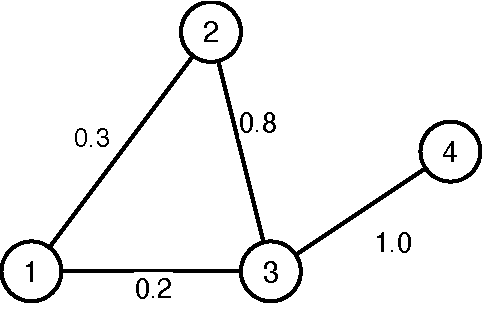
\includegraphics[width=0.4\textwidth]{images/weighted-unipartite.pdf}
	\caption{A weighted unipartite graph}
	\label{fig:weighted-unipartite-graph}
\end{figure}

For the graph in figure \ref{fig:weighted-unipartite-graph},
the vertices are $V = \{1, 2, 3, 4\}$.
The adjacency matrix is

\begin{equation*}
	A =
	\begin{bmatrix}
		0   & 0.3 & 0.2 & 0 \\
		0.3 & 0   & 0.8 & 0 \\
		0.2 & 0.8 & 0   & 1 \\
		0   & 0   & 1   & 0
	\end{bmatrix}
\end{equation*}

\textbf{Community detection problem}

In order to tell how good a community finding algorithm, one should use the \textit{quality function}.
It assign a score number to each partition of a graph.
By comparing the score of different partitions, one can tell which partition is better.
But keep in mind that, the answer for the question which partition is better is not universally
but depends on the specific concept of community adopted.

\textit{Modularity}\parencite{newman2004} is the most popular quality function in the literature.
The ideal is that, a random graph should not have any community structure.
By comparison the edge density of a subgraph and density of a similar random graph (or \textit{null graph}),
it is possible to reveal the community structure of the graph.
The modularity $Q$ can be defined as

\begin{equation}
	Q = \frac{1}{2m} \sum_{ij} \left(A_{ij} - P_{ij}\right) \delta(C_i, C_j)
\end{equation}

Where $m$ is the total number of edges in the graph,
$A$ is the adjacency matrix of the graph.
$P_{ij}$ is the probability that there is an edge between node $i$ and $j$ in a random graph.
The function $\delta$ is the Kronecker delta function,
which is 1 if $i$ and $j$ in a same community ($C_i = C_j$), and 0 otherwise.
Note that the sum is iterated over all pairs of nodes.
The choice of null graph is arbitrary, but it is common to use the configuration model \parencite{newman2004}.
This model consider two node $i, j$ with the degree $k_i, k_j$.
And the corresponding modularity is

\begin{equation}
	Q = \frac{1}{2m} \sum_{ij} \left(A_{ij} - \frac{k_i k_j}{2m}\right) \delta(C_i, C_j)
\end{equation}

One can group the contribution to the sum from the same clusters together,
to obtain the following form where the sum is iterated over all clusters instead of all pairs of nodes.
$n_c$ is the number of clusters, $l_c$ is the number of edges within cluster $c$ (the number of edges connecting vertices in cluster $c$),
$d_c$ is the sum of degree of all vertices in $c$.


\begin{equation}
	Q = \sum_{c=1}^{n_c} \left[\frac{l_c}{m} - \left(\frac{d_c}{2m}\right)^2 \right]
\end{equation}

There are some important properties of this modularity.
It is always smaller than one, and can be negative.
First, large positive values of modularity indicate good partitions \parencite{fortunato2010}.
Then, one should not use modularity to compare the goodness of partitions of two graphs that are very different in size.

In the case of weighted graph, the modularity can be written as

\begin{equation}
	Q_w = \frac{1}{2W} \sum_{ij} \left(A_{ij} - \frac{s_i s_j}{2W}\right) \delta(C_i, C_j)
\end{equation}

or the equivalent form

\begin{equation}
	Q_w = \sum_{c=1}^{n_c} \left[\frac{W_c}{W} - \left(\frac{S_c}{2W}\right)^2 \right]
\end{equation}

Here $W$ is the total weight of the graph, $W_c$ is the total weight of cluster $c$,
$S_c$ is the total strength of vertices in cluster $c$.

% \todo{resolution parameter}

The modularity is not a perfect quality function, researchers have found that it tend to ignore smaller communities \parencite{fortunato2007}.
Hence a parameter call \textit{resolution parameter} is introduced to overcome this problem.
Though modularity is not one-fit-all solution,
it is widely used in tools and libraries design for working with networks.
Scholars extended the concept of modularity to bipartite graph, which we will review in the next section.

\subsection{Bipartite graphs}

A bipartite graph is a graph where nodes are separated into two disjoint sets,
and links only exists between nodes of different sets.
Other name for this type of graph is two-mode networks, or affiliation networks.
Many real-world problem can be naturally modeled as bipartite graphs.
Some of the most famous examples are the movie-actor network, or the author-paper network.
In the movie-actor, the two sets of nodes are actors and movies.
An actor is connected to a movie if he/she play in that movie.
No links exist between actors, or between movies.
In the author-paper networks, there are only links between authors and papers,
happening when an author write a paper.

\begin{figure}[H]
	\centering
	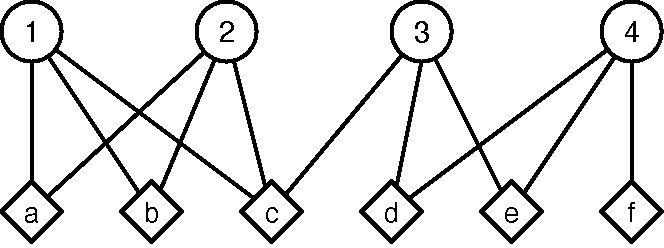
\includegraphics[width=0.4\textwidth]{images/unweighted-bipartite.pdf}
	\caption{An unweighted bipartite graph with two types of nodes: Int and Char}
	\label{fig:unweighted-bipartite-graph}
\end{figure}

Denote a bipartite network as $B(V_1 \cup V_2, E, \omega)$,
where $V1$ and $V2$ are the two disjoint sets of nodes: $V_1 \cap V_2 = \emptyset$.
The set of edges $E$ is a subset of $V_1 \times V_2$,
and the optional weight function $\omega$ is a function from $E$ to $\mathbb{R}$.
The number of nodes in $V_1$ is $n_1 = |V_1|$, and that for $V_2$ is $n_2 = |V_2|$.
The number of edges is $m = |E|$.
The average degree of the $V_1$ nodes is $k_1 = \frac{m}{n_1}$, of $V_2$ nodes is $k_2 = \frac{m}{n_2}$.
The average density of the bipartite graph is $\delta(B) = \frac{m}{n_1 n_2}$.
Note that this density is much lower than that of a unipartite graph with the same number of nodes $\frac{2m}{(n_1 + n_2)(n_1 + n_2 - 1)}$.

Bipartite graphs can be represented by the \textit{biadjacency matrix} $A$.
The matrix is of size $n_1 \times n_2$.
The element $A_{ij}$ is the weight of the edge between node $i$ and $j$.
For example the bipartite graph in figure \ref{fig:unweighted-bipartite-graph}
We have two set of nodes $V_1 = \{1, 2, 3, 4\}$ and $V_2 = \{a, b, c, d, e, f\}$.
Only nodes in different sets are connected together.
The biadjacency matrix is

\begin{equation*}
	A =
	\begin{bmatrix}
		1 & 1 & 1 & 0 & 0 & 0 \\
		1 & 1 & 1 & 1 & 0 & 0 \\
		0 & 0 & 1 & 1 & 1 & 0 \\
		0 & 0 & 0 & 1 & 1 & 1
	\end{bmatrix}
\end{equation*}

\textbf{Community detection problem}

In order to better describe the community problem in bipartite graph,
we employ the notation system from \parencite{pesantez2018} because of its simplicity.
We hereby recall some of the most important notations from the work.

In bipartite, a community is a subset of either $V_1$ or $V_2$.
Let $P_1 = \{C_1, C_2, \ldots, C_{p_1}\}$ is a partition of $V_1$,
where $C_i$ is a community in $V_1$.
Similarly, $P_2 = \{D_1, D_2, \ldots, D_{p_2}\}$ is a partition of $V_2$,
where $D_i$ is a community in $V_2$.
$p_1$ and $p_2$ are the number of communities in $V_1$ and $V_2$ respectively,
and they are not necessarily equal.


\textbf{One-mode \gls{project2}}

One-mode projection is a method to transform a bipartite graph into a unipartite graph.
Using such method, one can apply the well-developed notations and algorithms for unipartite graph to analyze the bipartite graph.
The one-mode projection onto $V_1$, or $V_1$-projection means create a network with only nodes in $V_1$,
two nodes in $V_1$ are connected if they share at least one common neighbor in $V_2$.
Mathematically, project a bipartite $B(U\cup V, E)$ to node set $V$
will yield a unipartite graph $G(V, E')$.

\begin{equation*}
	E' = \{(u, v) | u, v \in V, \exists w \in U, (u, w) \in E, (v, w) \in E\}
\end{equation*}

The result is simply an unweighted network that can not capture the frequency of connection in the original bipartite graph.
For example, Figure \ref{fig:Intprojection}, \ref{fig:Charprojection} corresponding shows the $V_1$-projection and $V_2$-projection of the graph in Figure \ref{fig:unweighted-bipartite-graph}.

\begin{figure}[H]
	\centering
	\begin{subfigure}[b]{0.4\textwidth}
		\centering
		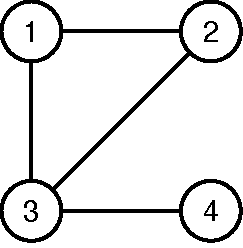
\includegraphics[width=0.5\textwidth]{images/bipartite-projection-number.pdf}
		\caption{Projection onto Int node}
		\label{fig:Intprojection}
	\end{subfigure}
	% \hfill
	% \hspace{1cm}
	\begin{subfigure}[b]{0.4\textwidth}
		\centering
		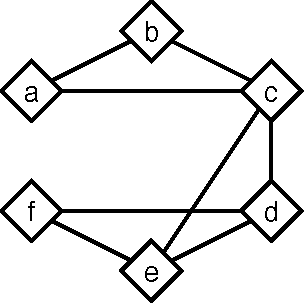
\includegraphics[width=0.5\textwidth]{images/bipartite-projection-char.pdf}
		\caption{Projection onto Char node}
		\label{fig:Charprojection}
	\end{subfigure}
	\caption{One-mode projection of the graph in Figure \ref{fig:unweighted-bipartite-graph}}
	\label{fig:projection}
\end{figure}

One-mode projection always contains less information than the original bipartite network.
Hence to better reflect the structure of the original network,
projected networks are often weighted.
Although there are many ways to weight the projected network,
the simplest way is to use the number of common neighbors as the weight.
Figure \ref{fig:Weightedprojection} shows that weighted projection of the graph in Figure \ref{fig:unweighted-bipartite-graph}.
Another famous weighting method is \textit{collaboration weight} or \textit{hyperbolic weight}
The idea is develop when author-paper bipartite network is under study.
In \parencite{newman2001}, Newman stated that if two authors only publish together only one paper,
then the two should be more connected than if they publish together 100 papers.
To reflect this idea, the weight is reduce by a factor of $1/(d_u-1)$
where $d_u$ is the number of author in considering paper, i.e. the degree of the paper node.

\begin{equation*}
	w_{v_1, v_2} = \sum_u \frac{\delta^u_{v_1}\delta^u_{v_2}}{d_u - 1}
\end{equation*}

Despite of the weighting method, the one-mode projection is still a lossy transformation.
In fact, it is one of the three main drawbacks of the projection.
The second one is, as quoted from \parencite{latapy2006},
"some properties of the projection may be due to the projection process rather than the underlying data itself".
For example, the projection of a not-very-dense bipartite network could be a very dense unipartite graph.
The third drawback, and perhaps it is the most difficult one to overcome when study large graph,
is the computational cost of the projection.
When project $B(V_1 \cup V_2, E)$ onto $V_1$,
each node in $V_2$ with degree $d$ will introduce $d(d-1)/2$ edges in the projected graph.
if the average degree of $V_2$ is high enough, the projection might be infeasible.

\begin{figure}[H]
	\centering
	\begin{subfigure}[b]{0.4\textwidth}
		\centering
		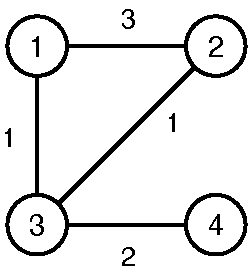
\includegraphics[width=0.5\textwidth]{images/weighted-bipartite-projection-number.pdf}
		\caption{Weighted Projection onto Int node}
		\label{fig:WeightedIntprojection}
	\end{subfigure}
	% \hfill
	% \hspace{1cm}
	\begin{subfigure}[b]{0.4\textwidth}
		\centering
		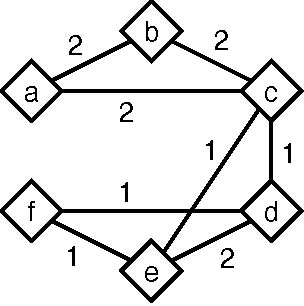
\includegraphics[width=0.5\textwidth]{images/weighted-bipartite-projection-char.pdf}
		\caption{Weighted Projection onto Char node}
		\label{fig:WeightedCharprojection}
	\end{subfigure}
	\caption{Weighted One-mode projection of the graph in Figure \ref{fig:unweighted-bipartite-graph}}
	\label{fig:Weightedprojection}
\end{figure}

\textbf{Directly detecting community in bipartite graph}

There are, however, method for directly detecting community in bipartite graph instead of projection.
Like in the unipartite case, quality functions is needed to judge the goodness of a community finding.
Literature try to extend to concept of modularity to bipartite graphs, which often call \textit{bimodularity}.
There are multiple efforts to define bimodularity, listed in \parencite{pesantez2018}.
They also employ the Murata's definition \parencite{murata2009} in their work because
it overcome the problem of enforcing one-to-one correspondence between communities in both vertex types.

The ideal of Murata's bimodularity is pairing every community $C$ from one vertex type with a community in the other vertex types
that it has maximum connection to.
This is also call \textit{co-cluster mate} of community $C$, denoted by $\psi(C)$.
\begin{equation}
	\psi(C) = \argmax_{D \in P_e} \mathcal{E}_{C, D}
\end{equation}

In which, define
\begin{equation}
	\mathcal{E}_{C, D} = \frac{1}{W} \sum_{e} \omega (e)
\end{equation}
$e$ denotes any edges between two vertices community $C\in P_1$ and $D\in P_2$.
And the fraction of this term contributed by all vertices in community $C$ is

\begin{equation}
	\mathcal{A}_C = \frac{1}{W} \sum_{D} \mathcal{E}_{C, D}
\end{equation}

\begin{figure}[H]
	\centering
	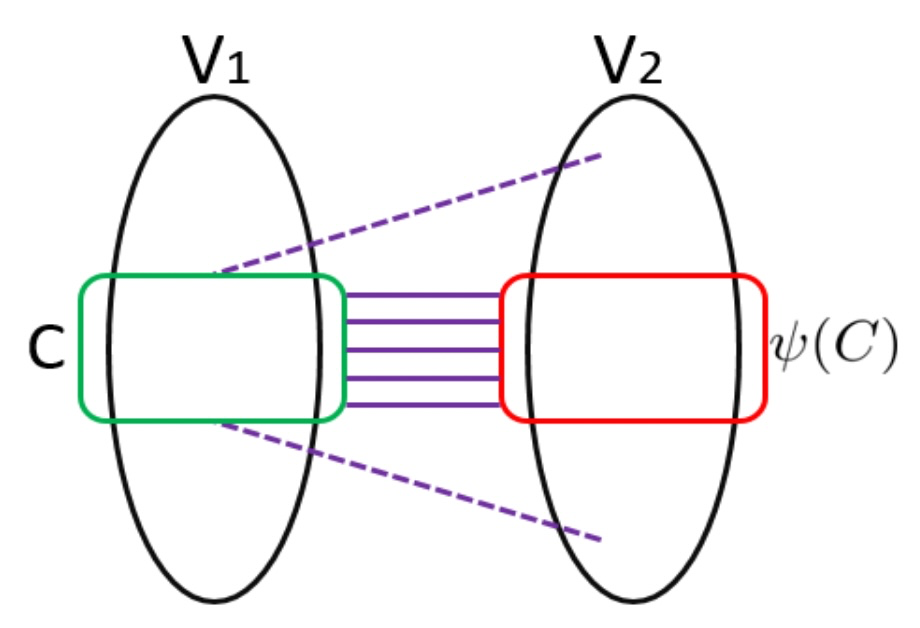
\includegraphics[width=0.4\textwidth]{images/cocluster.png}
	\caption[Illustration of a co-cluster]{
		Illustration of a co-cluster
		$\langle C, \psi(C) \rangle$
		where $\psi(C)$ is referred as the co-cluster mate of community $C$,
		reprinted from \parencite{pesantez2018}
	}
	\label{fig:co-cluster}
\end{figure}

Given those definition, then the Murata bimodularity $Q_B$ is

\begin{equation}
	\label{eq:murata-bimodularity}
	Q_B = \sum_C \left(\mathcal{E}_{C, \psi(C)} - \mathcal{A}_C \times \mathcal{A}_{\psi(C)}\right)
	+ \sum_D \left(\mathcal{E}_{D, \psi(D)} - \mathcal{A}_D \times \mathcal{A}_{\psi(D)}\right)
\end{equation}

\begin{figure}[H]
	\centering
	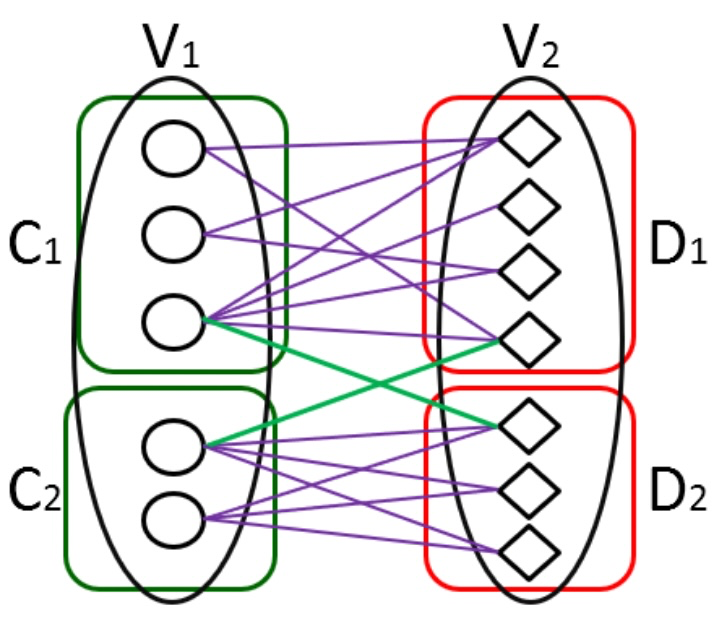
\includegraphics[width=0.4\textwidth]{images/cocluster2.png}
	\caption[Illustration of co-clusters]{
		Illustration of co-clusters, reprinted from \parencite{pesantez2018}
	}
	\label{fig:cocluster2}
\end{figure}


The work of \parencite{pesantez2018} provides some observations regarding the Murata metric.
And then proposed a new metric called \textit{Murata+} to overcome the drawbacks of the original Murata metric.

The Murata+ still use the same definition as in equation \ref{eq:murata-bimodularity}.
But in which, change the co-cluster mate definition to

\begin{equation}
	\psi(C) = \argmax_D \left(\mathcal{E}_{C, D} - \mathcal{A}_C \times \mathcal{A}_D\right)
\end{equation}

The work claim several advantages of the Murata+ metric and it is well-suited for identifying significant communities in bipartite networks.

\textbf{The biLouvian algorithm}

In this thesis, we faced a unsupervised problem, hence the main focus is to build a good methodology to find community and evaluate the result.
There are many algorithms for community detection problem directly in bipartite graph \parencite{pesantez2018}.
Reviewing and testing all the algorithms is not possible within the scope of this thesis.
We will focus on the \textit{biLouvian} algorithm \parencite{pesantez2018} for detecting community directly in bipartite graphs
because of its characteristics: deterministic, produce co-cluster mate,
and the fact that the authors claim that it is outperform other algorithms in their experiments.
The deterministic is important because in the later propose methodology,
we will run the algorithm multiple times to find.
The algorithm mimic the idea from the Louvian algorithm \parencite{blondel2008}, hence the name.
It try to optimize the Murata+ bimodularity metric by assign nodes to various communities and find the best metric value.
We do not go into the detail of the algorithm.


\begin{figure}[H]
	\centering
	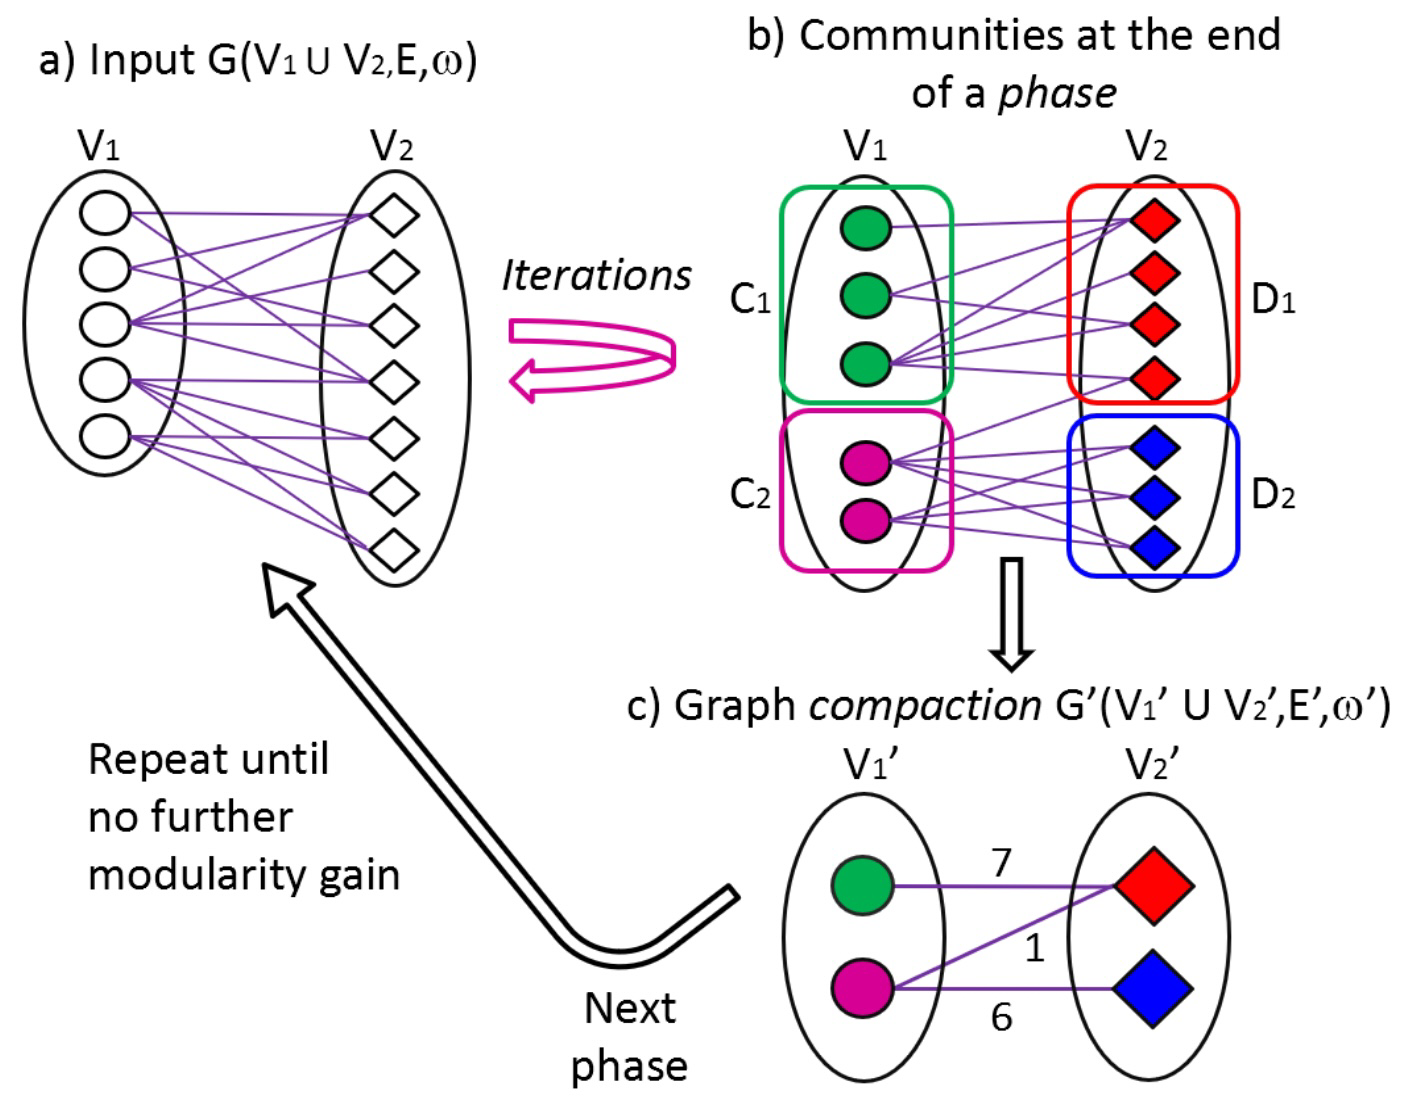
\includegraphics[width=0.6\textwidth]{images/biLouvian-algorithm.png}
	\caption{Main steps of biLouvian algorithm, reprinted from \parencite{pesantez2018}}
	\label{fig:biLouvian-algorithm}
\end{figure}



%Conclusion for the Literature review, and transition to the next section

In this chapter, we review the crowdfunding problem and the community detection problem.
Both of these problems are still under active research.
In crowdfunding, the dynamics and factors that drive the successfulness of a campaign are not well understood.
While in community detection, there are no universally accepted, no one-fit-all definition and algorithms.
In following chapters, we will propose a methodology to study the dynamics of crowdfunding campaigns using community detection problem.
But first, we will introduce the dataset that we use in the next chapter.


\begin{comment}
\subsection{plan}
\begin{itemize}
	\item Definition of community finding on a graph
	      Perhaps the most famous literature on community finding is \parencite{fortunato2010}
	      But a quote from the paper
	      This problem is very hard and not yet satisfactorily solved, despite the huge effort of a large interdisciplinary community of scientists working on it over the past few years.
	\item In real networks, the usually exist a group of vertex that have high density of connection between them,
	      but lower density of connection with the rest of the network.
	      This group of vertex is called community structure or clustering.
	      The community finding problem is to find these group of vertex.
	\item Community finding is a very important problem in network science.
	      Because vertex in community usually share similar properties, or play a similar role in the graph

	\item Community finding is a hard problem
	      \parencite{fortunato2010} show that it is a NP-hard problem
	\item Community finding on dynamic graph
	      \begin{itemize}
		      \item The static graph community analysis is already controversial
		            Hence not much work on dynamic graph
	      \end{itemize}
	\item Testing algorithms
	      \begin{itemize}
		      \item *planted l-partition model* \parencite{fortunato2010}
		      \item
	      \end{itemize}
	      \begin{itemize}
		      \item Most of the works focus on develop algorithms to find community, benchmark on supervised datasets
	      \end{itemize}
	\item Review community finding on
	      \begin{itemize}
		      \item unipartite graph (most of literatures): annotations, algorithms, metrics
		      \item bipartite graph: annotations, algorithms, metrics, projection methods
		      \item Very rate 3-partite graph: just listing the works
	      \end{itemize}

\end{itemize}
\end{comment}